\documentclass[11pt, oneside]{article} 
\usepackage{geometry}
\geometry{letterpaper} 
\usepackage{graphicx}
	
\usepackage{amssymb}
\usepackage{amsmath}
\usepackage{parskip}
\usepackage{color}
\usepackage{hyperref}

\graphicspath{{/Users/telliott/Github/precalculus/fig/}}
% \begin{center} \includegraphics [scale=0.4] {gauss3.png} \end{center}

\title{Perpendicular bisector}
\date{}

\begin{document}
\maketitle
\Large

\subsection*{altitude of an isosceles triangle}

Consider this triangle with two equal sides --- isosceles.
\begin{center} 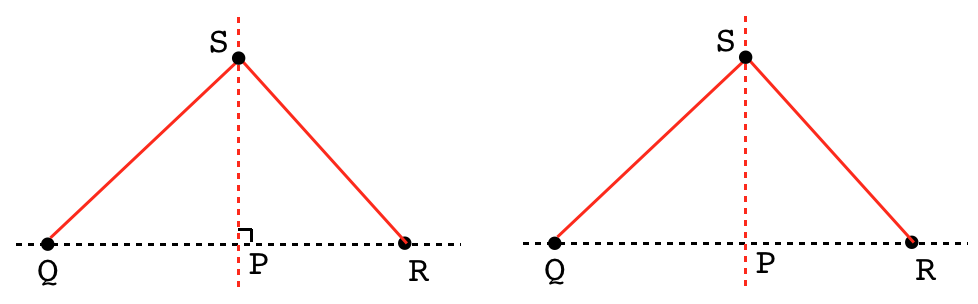
\includegraphics [scale=0.35] {isosceles3.png} \end{center}
If we are given $QS = SR$, by the theorem on isosceles triangles, we know that the base angles  $\angle PQS$ and $\angle PRS$ are equal (Euclid \hyperref[sec:Euclid5]{\textbf{Prop $I.5$}}).

Alternatively, if the base angles are equal, then so are the sides (Euclid \hyperref[sec:Euclid6]{\textbf{Prop $I.6$}}).

If $\angle SPR$ is a right angle, then the $SP$ bisects the base as well as the vertex $\angle QSR$.

Proof.

We have two equal angles in the smaller triangles, plus a shared side (AAS).  

Therefore $\triangle QPS \cong \triangle PRS$, so the segments on the base are equal.  

$QP = PR$.

$\square$

If the base is bisected, above, then the line segment $SP$ is an \emph{altitude} of the triangle, and it meets the base in a right angle.

Proof.

We are given that $QP = PR$.  Then $\triangle QPS \cong \triangle PRS$ by SSS. 

Therefore $\angle QPS = \angle SPR$ and both are right angles by the supplementary angles theorem (\hyperref[sec:supplementary_angle_theorem]{\textbf{ref}}).

$\square$

\subsection*{bisector is the altitude of an isosceles triangle}

Suppose we know two points $Q$ and $R$.  We find the point $P$ equidistant between them and construct the perpendicular bisector $PS$.  Then the two sides $SQ$ and $SR$ have equal length.  Triangle $\triangle SQR$ is isosceles.

\begin{center} 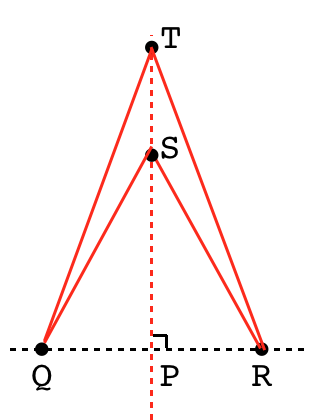
\includegraphics [scale=0.45] {perp_3.png} \end{center}

Proof.  By the theorem from above.

This is true for \emph{any} point on the line drawn through $S$ and $P$.  For example, $TQ = TR$ in the figure above.

\subsection*{to construct a perpendicular bisector}

Suppose we wish to construct a line segment perpendicular to another line segment.  There are three common situations (see the figure below):

- We want the bisector to pass through a given point $P$ on the line.

- We know points $Q$ and $R$ on the line and want the bisector to pass halfway between them

- We want the bisector to pass through a point $S$ not on the line

\begin{center} 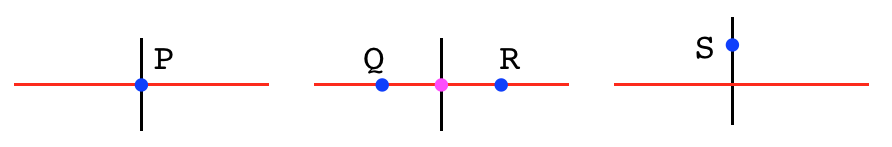
\includegraphics [scale=0.4] {perp8.png} \end{center}

We solve the second case and then show how the other two can be adapted to it.

\subsection*{bisector between two points}

Simply construct two circles of equal radius, one centered at $Q$ and the other at $R$.  It's easiest to choose the radius to be equal to the length $QR$ (left panel, below).

\begin{center} 
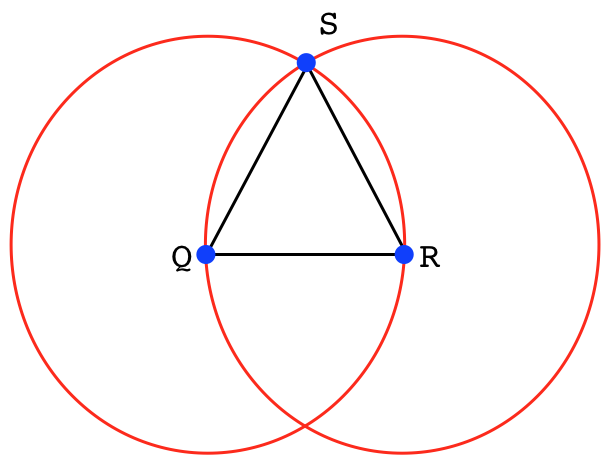
\includegraphics [scale=0.3] {perp9.png} 
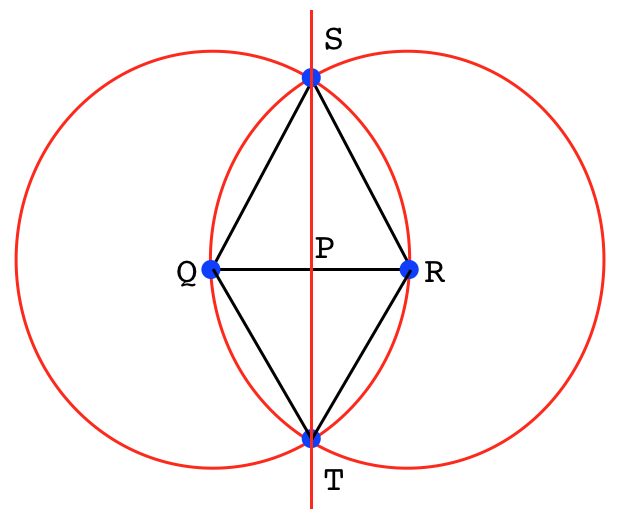
\includegraphics [scale=0.3] {perp10.png} 
\end{center}

The point $S$ is on both circles, hence it is a radius of both, and therefore equidistant from $Q$ and $R$.  $QS = SR = QR$.  

The three points form an equilateral triangle, $\triangle QRS$ (Euclid \hyperref[sec:Euclid1]{\textbf{Prop $I.1$}}).

The point $T$ below the line segment has the same property, and $\triangle QRS$ is congruent to $\triangle QRT$ by SSS.

The line segment $ST$ is perpendicular to $QR$ and the point $P$ where $ST$ intersects $QR$ is such that $QP = PR$.

Proof.

$\circ$ \ $\triangle QST \cong \triangle SRT$ by SSS (two equal and one shared).

$\circ$ \ Therefore the two angles at $S$, $\angle QSP$ and $\angle PSR$, are equal. 
 
$\circ$ \ Therefore $\triangle QPS \cong \triangle PRS$ by SAS.

$\circ$ \ $QP = PR$ by congruent $\triangle$.

$\circ$ \ $\angle QPS = \angle SPR$ by congruent $\triangle$, so both are right angles.

$\circ$ \ Therefore all the angles at $P$ are right angles.

$\square$

\subsection*{bisector through a given point on the line}

Suppose we know a point $P$ on the line and wish to construct the vertical line through $P$.  

Use the compass to mark off points $Q$ and $R$ on both sides of $P$, equidistant from it.  This can be done by drawing a circle with center at $P$.

\begin{center} 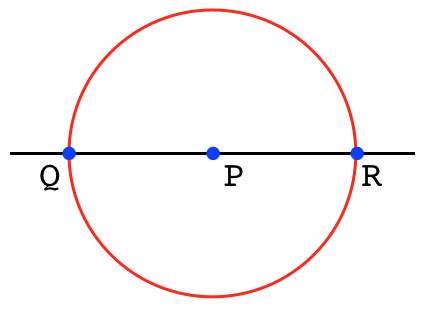
\includegraphics [scale=0.4] {perp_7.png} \end{center}

Now, simply proceed as above.

\subsection*{bisector through a given point not on the line}

Alternatively, suppose we know the line and the point $U$ but not $P$, and we wish to construct a vertical through the line that also passes through $U$.  

Find $Q$ and $R$ on the line an equal distance from $U$ ($QU$ = $RU$), as radii of a circle centered at $U$ (left panel, below).  Their exact position is unimportant.  

\begin{center} 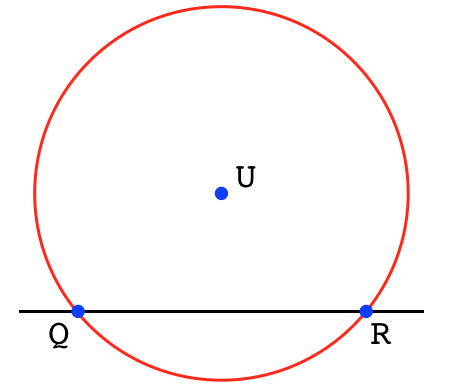
\includegraphics [scale=0.35] {perp11.png} \end{center}

Now repeat the previous construction, using $Q$ and $R$.  The line segment $ST$ pass through $U$, as required.

Proof.

(Sketch).  Since $QU = RU$, $\triangle QUR$ is isosceles.  Therefore the base angles are equal.  In an isosceles triangle, the top vertex lies on the perpendicular bisector of the base (see the first part of this chapter).

\subsection*{collapsible compass}

We note briefly that there is a restriction in Euclid's \emph{Elements} to a \emph{collapsible} compass, one which loses its setting when lifted from the page.  That means that generally, you wouldn't be able to draw two circles of the same radius on different centers.

We get around that restriction by drawing the circles on $Q$ and $R$ with the same radius $QR$.  

We will call a compass that is able to hold its setting, a \emph{standard} compass, and explain why the distinction is important to Euclid in the chapter devoted to his book.  Within the first few pages of that book, it is shown how to use a collapsible compass to carry out the very construction we said we couldn't do, namely, construct two circles on $Q$ and $R$ with equal radius and that radius not equal to $QR$ or $QP$.

Also, see the video at the url:

\url{https://www.mathopenref.com/constperpextpoint.html}

\subsection*{three points}

Now, suppose we have three points:  $Q$, $R$ and $S$.  We find the perpendicular bisector of $QR$ and also, the perpendicular bisector of $QS$.  Extend them to where they meet, at point $O$.

\begin{center} 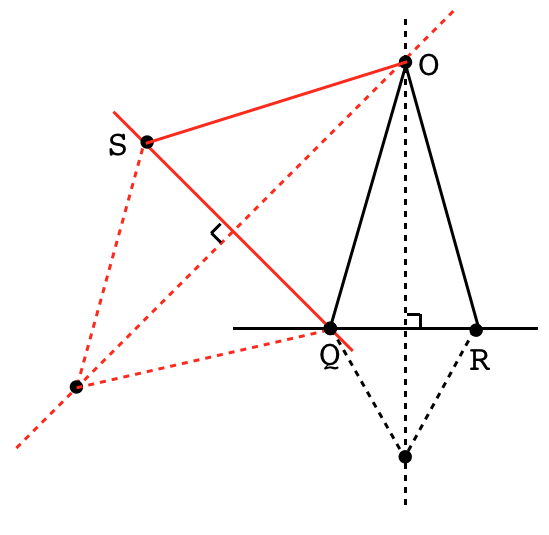
\includegraphics [scale=0.35] {perp_4.png} \end{center}

What can we say about point $O$?

$\circ$ \ $O$ is equidistant from $Q$ and $R$.

$\circ$ \ $O$ is also equidistant from $Q$ and $S$.

Therefore, $OQ = OR = OS$.  If we draw a circle on center $O$ with radius $OR$, it will pass through all three points.

\begin{center} 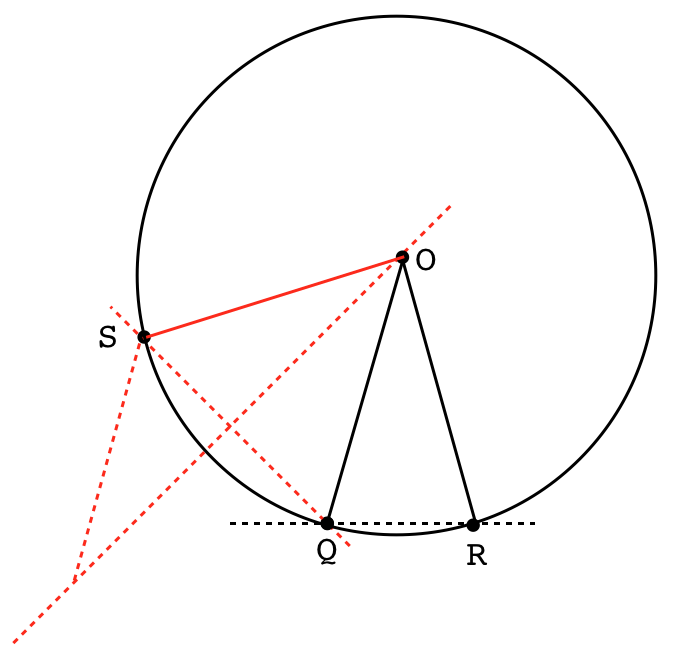
\includegraphics [scale=0.3] {perp_5.png} \end{center}

\subsection*{circumcenter}

The point where the perpendicular bisectors cross has a special name, it is called the circumcenter.

\begin{center} 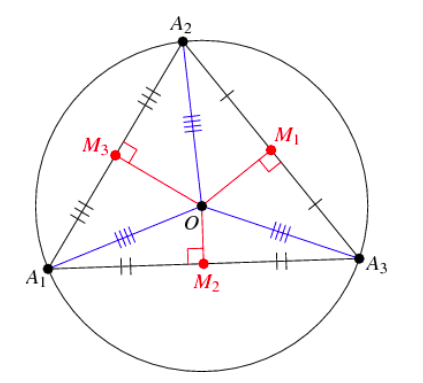
\includegraphics [scale=0.5] {three_point_circle2.png} \end{center}

There are other special points where interesting circles can be drawn.

\subsection*{circumscribed circle}

Here is a fun construction based on an equilateral triangle.  

Any triangle fits into a unique circle (see above).
\begin{center} 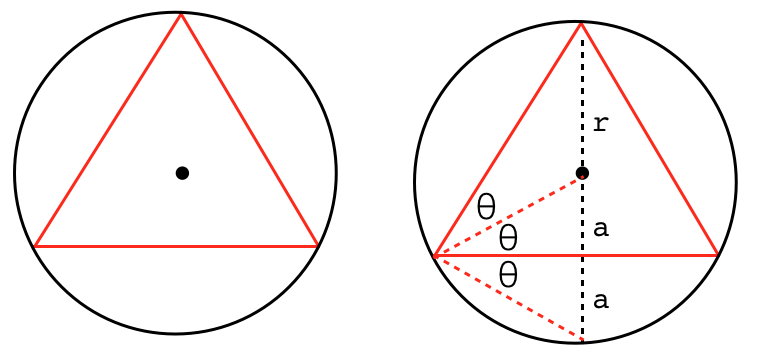
\includegraphics [scale=0.4] {one_third.png} \end{center}

Draw the radius to a vertex of the triangle, and extend it as the diameter.  We will show that the three angles marked $\theta$ are equal.

Proof.  

The perpendicular bisector of an isosceles (or equilateral) triangle is an altitude and it goes through the center of the circle containing all three vertices.

It divides the vertex angle in half, as we've been saying.  So that accounts for two of the angles labeled $\theta$.  

The third comes about because any triangle with two points at the ends of the diagonal and a third anywhere on the circle is a right triangle.  We'll prove that when we get to circles.

As a result,  $\theta$ measures $30$ degrees.  Since a right triangle is $90$ degrees total, we assign the third $\theta$.

\begin{center} 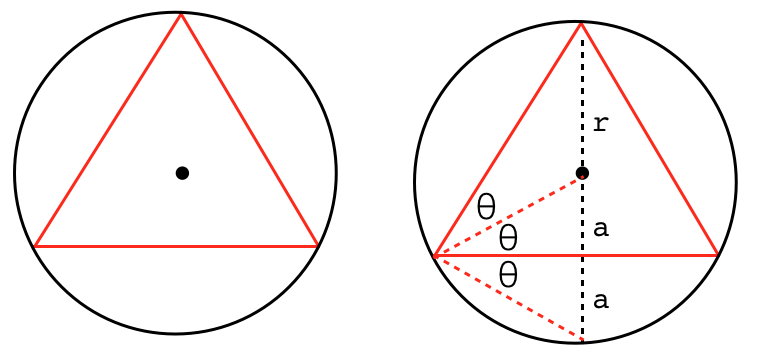
\includegraphics [scale=0.4] {one_third.png} \end{center}

So now we have one of the complementary angles of a right triangle, and a shared side.  The two triangles are congruent.  That accounts for the duplicated $a$ in the figure.

Thus, the altitude of the equilateral triangle is $3/4$ of the diameter of the circle that just encloses it.  And the point where the altitudes meet in an equilateral triangle is $1/3$ of the way up from the base, since $r = 2a$.  

We will see that such a point where the altitudes cross is unique and exists for any triangle, and it always has the same measure as a fraction of the altitude.  This is called Ceva's theorem.


\end{document}